\documentclass{standalone}

\usepackage[OT1]{fontenc}
\renewcommand*\familydefault{\sfdefault}
\usepackage{helvet,sfmath}
\usepackage{siunitx}

\usepackage{tikz}
\usetikzlibrary{arrows,calc,patterns}
\usepackage{tikz,tkz-euclide}
\usepackage{circuitikz}

%% Color %%
\definecolor{BlueDefault}{rgb}{0.2,0.2,0.7}
\definecolor{Fr4}{RGB}{228, 188, 65}
\definecolor{Copper}{RGB}{184, 115, 51}

\begin{document}

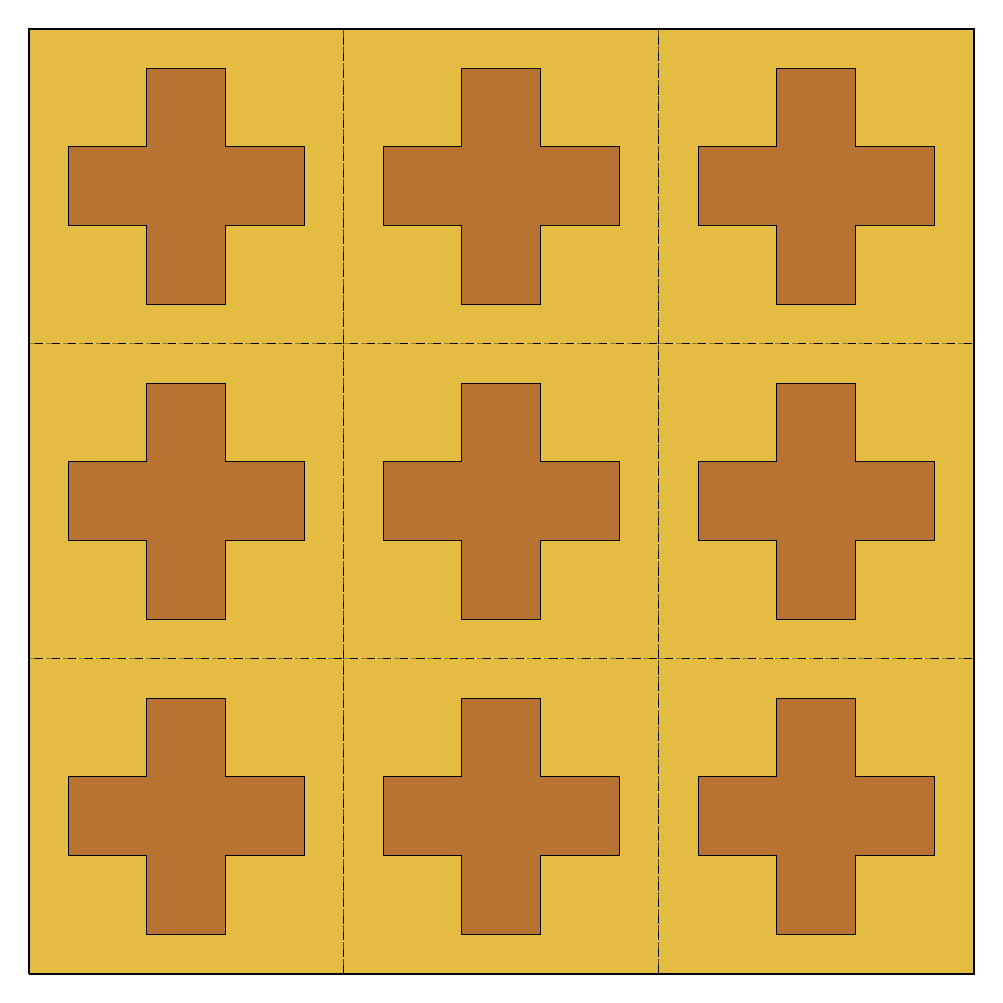
\begin{tikzpicture}[scale=1]
    \foreach \x in {-4,0,4}
    \foreach \y in {-4,0,4}
    {
    \draw[dashed, fill = Fr4] (\x-2,\y-2) to (\x-2,\y+2) to (\x+2,\y+2) to (\x+2,\y-2) to (\x-2,\y-2);
    \draw[fill = Copper] (\x-0.5,\y-0.5) to (\x-0.5,\y-1.5) to (\x+0.5,\y-1.5) to (\x+0.5,\y-0.5) to (\x+1.5,\y-0.5) to (\x+1.5,\y+0.5) to (\x+0.5,\y+0.5) to (\x+0.5,\y+1.5) to (\x-0.5,\y+1.5) to (\x-0.5,\y+0.5) to (\x-1.5,\y+0.5) to (\x-1.5,\y-0.5) to (\x-0.5,\y-0.5);
    }
    \draw[thick] (-6,-6) to (6,-6) to (6,6) to (-6,6) to (-6,-6);
\end{tikzpicture}

\end{document}

